\chapter{The Mathematics}
\label{ch:07}



\begin{center}
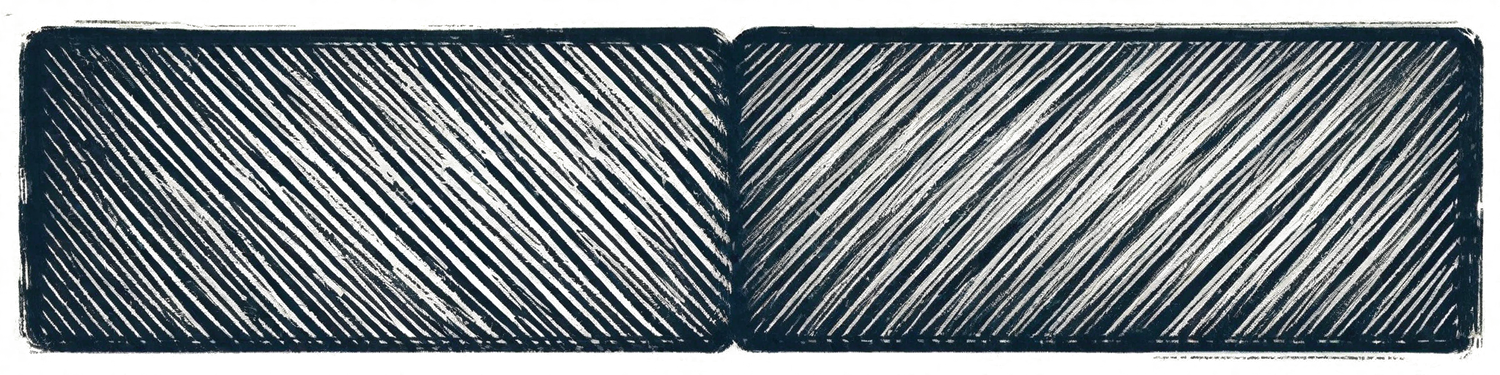
\includegraphics[width=\textwidth]{images/chapterImages/genesis_sketch_00074_.png}
\end{center}

The wrongstar was visible during daylight now. Not bright enough to hurt to look at, but present. A pale point in the blue sky that shouldn't exist. Every rotation it was more obvious. Every observation confirmed the calculations with increasing precision.

1,847 rotations remaining.

Aurelia's pattern had grown to encompass most of the clearing and extended into the forest beyond. Stones of every size marked positions in a three-dimensional grid that existed partly in physical space and partly in the conceptual space behind her eyes. To walk through it was to walk through mathematics made tangible.

She spent more time still than moving now. Days would pass where she stood in one position, breathing perhaps twice per minute, eyes fixed on nothing or everything, while behind them entire evolutionary timelines unfolded and tested themselves against probability.

The young ones were almost adult now. They hunted independently. They understood the protection work without needing guidance. They added their own stones to the pattern with increasing accuracy. The youngest—the female—had begun her own smaller pattern adjacent to the main one, her mathematics simpler but sound.

And the other one remained. His roost had become permanent. His hunting range had merged with hers. His pattern work complemented hers. They existed in parallel, their mathematics intersecting at key points, creating a whole that exceeded the sum of parts.

He brought food when she was too deep in calculation to hunt. She would find it cached near the pattern's edge, always fresh, always sufficient. She consumed it mechanically and returned to stillness. The reciprocity was functional. Necessary. Efficient.

Nothing more than that needed to be named.

\scenebreak

She was standing in her observation position—had been standing there for six days now, processing a particularly complex section of the probability tree—when the sound came.

Not a cry. Not a call. Just impact. The heavy thud of a body hitting earth. The scatter of disturbed stones. Then silence.

She came out of the calculation slowly, like surfacing from deep water. The transition from mathematical space to physical space took several seconds. When her awareness finally settled into her body, she moved.

He was at the pattern's edge, where a steep slope descended toward the river. A section where large stones needed positioning, where the footing was treacherous. He had been moving one of the massive rocks, leveraging it into place using his weight and the fulcrum of a branch.

The branch had broken. Or his footing had failed. The specific mechanism didn't matter.

He lay on his side at the bottom of the slope, partially beneath the stone he had been moving. His breathing was shallow. Blood ran from his snout where the fall had torn skin. One leg angled wrong.

She approached carefully. Assessed. The leg was broken. The internal injuries were unclear but probable. He was conscious, eyes tracking her approach, but he didn't try to rise.

In his mouth, still clenched in his teeth, was a small mammal. Fresh-killed. He had been hunting for her while also working on the stone placement. Attempting to do both simultaneously.

She looked at the mammal. Looked at him. Looked at the stone half-positioned, the pattern disrupted, the mathematics incomplete.

Ran calculations automatically: Survival probability. Recovery timeline. The cost in rotations of healing versus the cost in rotations of death. Whether the work could continue without him. Whether his contributions were necessary or merely supplementary.

The mathematics said: supplementary. The work could continue without him. The survival probability for the project decreased by less than three percent with his loss. Acceptable variance. Within tolerable parameters.

She stood over him while these calculations completed. He watched her with those amber eyes that had become familiar. Didn't make sound. Didn't display distress beyond the obvious physical damage.

Then she settled down beside him.

Not touching. Not providing aid—there was no aid to provide. She couldn't set the broken bone. Couldn't stop internal bleeding. Couldn't reverse impact trauma. She simply settled into a sitting position three body lengths away and stayed there.

The young ones found them that evening. They approached carefully, confused by the stillness, by the disruption to normal pattern. The female chirped questioningly. Aurelia didn't respond.

They investigated the fallen one from a distance, sensing injury, sensing the stillness that meant decline. The smallest one brought food and left it near the Watcher. She didn't acknowledge it.

They retreated to their hollow eventually, uncertain but surviving. That was what they did. What they were learning to do. Survive without constant guidance. Without her attention. This was useful training, though not deliberately designed.

The first night, he was still breathing. She could hear it in the darkness. Shallow but present. She didn't sleep. Didn't move. Just listened to that breathing and ran calculations that had nothing to do with projects or timelines or survival probabilities. Calculations that refused to resolve. Variables that wouldn't stabilize. Mathematics that led nowhere.

By dawn, his breathing had worsened. More labored. Rattling in the chest that meant fluid accumulation. Infection, probably. Internal damage. The inevitable cascade of system failure.

She should have returned to work. The pattern needed completion. The mammals needed protection. The young ones needed final instruction. Every rotation mattered.

She didn't move.

The second day passed with heat and insects and the distant sounds of the forest continuing its patterns without them. Other dinosaurs moved through the territory but didn't approach. Something in the configuration of two still figures, one dying, signaled do not disturb in language beyond words.

The tool-using mammal emerged from its burrow, used its modified stick to forage, returned safely. The work she had begun continued without her attention. The probability trees extended themselves another day forward.

She watched none of it. Watched only the slow rise and fall of his breathing. Counted the intervals. Noted when they lengthened. When they became irregular. When they stopped being something that could be called breathing and became something else. The space between alive and not alive, stretched thin.

By the third morning, he wasn't breathing.

She sat with the body for another hour after the breathing stopped. Making certain. Confirming the absence of function. Running no calculations because no calculations were relevant. He was matter now. Just matter. The complexity that had been thought and movement and contribution had ceased. The physics remained but the mathematics—the particular equations that had defined him as an individual process—those had terminated.

She stood eventually. Stiff from three days of motionless sitting. Her own body needed water, food, movement. The work needed continuation. The timeline didn't pause for individual terminations.

She moved to the pattern. Found the stone he had been trying to place. It had rolled slightly in the fall but was intact. She examined its position, calculated the original intent, understood what he had been trying to achieve.

She moved the stone to its correct position. It was too heavy for her alone—she had to lever it using the same technique he had attempted, but with better footing, with care for the angle and stress point. It took most of the morning, but she positioned it correctly.

Then she returned to the body and sat for another hour.

The young ones approached cautiously. The female chirped again. Aurelia made a sound back—an acknowledgment but not instruction. The young ones understood as much as they were capable of understanding. The other one who had been present was no longer present. The work continued anyway.

They needed to eat. Aurelia led them to hunt. They brought down prey efficiently, their technique refined by months of practice. She watched them eat. Consumed some herself. The mechanical requirement of survival satisfied.

Then she returned to the body.

This pattern continued for days. Work in the morning. Sit with the body in the afternoon. Hunt with the young ones when necessary. Return to the body. No logic dictated this pattern. The mathematics didn't justify it. The timeline didn't allow for it.

She did it anyway.

Other creatures came to investigate the body. Scavengers sensing opportunity. She drove them away. Not aggressively. Just her presence was sufficient to redirect them. The body remained undisturbed except by insects and the gradual process of decay.

She didn't bury it. Their kind didn't bury. Death was return to matter, recycling of elements. The body would be consumed by smaller things, incorporated into other life, dispersed through the system. This was normal. Natural. Efficient.

She prevented it for seventeen days.

The body became landscape. Flesh receded. Bone emerged. Feathers loosened and scattered. The smell shifted from fresh death to aged death to something else. Transformation. The same molecules rearranging themselves into different configurations. Life becoming not-life becoming different-life.

She watched it happen with the same intensity she had watched the tool-using mammal. Tracking each stage. Noting each transition. Learning nothing useful. Gaining no advantage for the project. Wasting rotations that were measured and finite.

On the eighteenth day, she moved a stone to mark the location. Not part of the pattern. Not encoding data. Just a stone placed where the body was. Had been. Was becoming something else.

Then she returned to work.

The pattern section he had been completing—she finished it. Not exactly as he would have. Her mathematics was more complex, her projections reached farther forward. But she maintained the fundamental structure he had established. Built on his foundation rather than replacing it.

Where his calculations had documented baseline environmental conditions, she extended them to show how those conditions would shift post-impact. Where he had encoded survival thresholds, she added recovery timelines. The pattern became synthesis. Collaboration across the termination of one participant.

She worked now with an intensity that burned through her remaining reserves. Calculations that had taken days before she processed in hours. The pattern exploded outward in complexity and scope. She barely ate. Barely slept. The young ones brought her food and water and she consumed it without awareness. Her body became almost incidental. Just the mechanism that held the mind that ran the mathematics.

The mammals continued under protection. The tool-user had offspring who were learning tool use. The second generation of selected traits. The probability trees branching forward exactly as calculated. The work was succeeding.

She was succeeding.

And she was alone in a way she hadn't been for months. The work continued. The mathematics held. But something had changed that mathematics couldn't quantify. Some variable that shouldn't exist but did. Some factor that the calculations couldn't incorporate because it had no numerical value.

She stood sometimes where he had worked. Placed stones where he would have placed them. Ran calculations from his perspective, simpler than hers but sound. Maintained his section of the pattern even as she expanded her own.

The body became mostly skeleton. Then mostly not-there. The insects and bacteria and patient decay did their work. Eventually, only the largest bones remained, half-buried in disturbed soil. The stone she had placed stood nearby.

She walked past it multiple times per day. Never stopped. Never looked directly at it. But her path always routed through that specific location. Always brought her within sight of the marked spot.

1,654 rotations remaining.

The young ones were fully adult now. They would breed soon. They might have their own young before the impact. That was acceptable. Good, even. More distributed intelligence to carry the knowledge forward if any of them survived.

The female had completed her sub-pattern. The mathematics was sound, if limited in scope. She was ready to work independently. To contribute without supervision.

All three of them were ready. They didn't need the Watcher anymore, not really. They could hunt, work, protect, survive. Everything she had taught them through demonstration and necessity had taken root.

And still the Watcher continued. Not for them. For the project. For the timeline. For the calculations that said maybe, just barely, survival was possible.

She stood in the pattern's center one evening and looked at the wrongstar, now bright enough to cast faint shadows at night. Looked at the stone pattern sprawling in every direction, the mathematics made physical. Looked toward where the body had been, where only a marked stone remained.

Ran calculations that included his contributions. That accounted for the work he had completed. That recognized his role in increasing success probability by three percent—a number that seemed trivial but over millions of rotations cascaded into significance.

His matter was dispersed now. His mathematics remained.

That was sufficient. Had to be sufficient.

She picked up the next stone. Placed it in the position the calculations demanded. The pattern grew. The work continued. The timeline advanced toward its inevitable endpoint.

And she did not stop. Did not pause again. Did not waste another rotation on things that didn't advance the probability of success.

The mathematics was complete. The hesitation was over. The work consumed everything now until it was finished or she was.

1,654 rotations remaining. She would use every single one.

